\section{Analysis}

\subsection{Analytical}

This section will detail the time complexity of each method.\\

\begin{table}[t]
\centering
\begin{tabular}[t]{| l | l |}
	\hline
	\multicolumn{2}{| c |}{\code{RedBlackTree}} \\ \hline
	\textbf{Method} & \textbf{Time complexity} \\ \hline
	\code{isEmpty()} & O(1) \\ \hline
	\code{contains(Object)} & O(log n) \\ \hline
	\code{hasPredecessor(Object)} & O(1) \\ \hline
	\code{hasSuccessor(Object)} & O(1) \\ \hline
	\code{predecessor(Object)} & O(log n) \\ \hline
	\code{successor(Object)} & O(log n) \\ \hline
	\code{min()} & O(1) \\ \hline
	\code{max()} & O(1) \\ \hline
	\code{add(Object)} & O(log n) \\ \hline
	\code{delete(Object)} & O(log n) \\ \hline
	\code{iterator()} & O(1) \\ \hline
	\code{iterator(Object)} & O(log n) \\ \hline
	\code{toString()} & O(n) \\ \hline
\end{tabular}
\begin{tabular}[t]{| l | l |}
	\hline
	\multicolumn{2}{| c |}{\code{TreeIterator}} \\ \hline
	\textbf{Method} & \textbf{Time complexity} \\ \hline
	\code{hasNext()} & O(1) \\ \hline
	\code{next()} & O(log n) \\ \hline
	\code{remove()} & O(log n) \\ \hline
\end{tabular}
\caption{Summary of time complexity of each method.}
\end{table}

Red-black trees have five main properties:
\begin{enumerate}
\item A node is either black or red.
\item The root node is black.
\item Every leaf node is black.
\item A red node has black children.
\item Every path from a node to a leaf descendent contains the same number of black nodes.
\end{enumerate}

Since the height of the tree is referenced in demonstrating the worst-case time complexity of almost every method in the class, I first prove the following limit on the height of a red-black tree \cite{clrs}:
\begin{equation*}
h \leq 2\log_2(n+1)
\end{equation*}
\begin{proof}
To begin, we prove that a subtree with root node $n$ has a minimum of $2^{h_b(n)} - 1$ internal nodes (where $b_h(n)$, the `black-height' of $n$, is the number of black nodes on any path from the node $n$ to any leaf, not including $n$): we do this by induction. For the base case - if the black height of $n$ is zero, then $n$ must be a leaf - and so $2^0 - 1 = 0$ is the number of internal nodes. So it holds for $b_h(n) = 0$. Now we assume that a node $n$ has a positive height and two children (i.e. $n$ is an internal node). Then each child must have a height of $b_h(n)$ or $b_h(n) - 1$, depending on the colour of the child. We can then apply the inductive hypothesis to the children - then each child has $2^{b_h(n) - 1} - 1$ internal nodes. Therefore we can simply sum the number of internal nodes of the two child subtrees to prove the claim - the subtree rooted at $n$ will have at least $(2^{b_h(n) - 1} - 1) + (2^{b_h(n) - 1} - 1) + 1 = 2^{b_h(n)} - 1$ internal nodes.

With the above combined with red-black tree properties, we can complete the proof: if we have a tree of height $h$, then according to the fourth property of red-black trees, at least half of the nodes on any path from the root to a given leaf (not including the root) are black. So $b_h(r) \geq \frac{h}{2}$, where $r$ is the root node of the tree. Then $n \geq 2^{\frac h 2} - 1$, and $h \leq 2\log_2(n + 1)$ follows.
\end{proof}

\subsubsection{\code{isEmpty()}}
This method performs a single null-check of the root node and is independent of the number of elements in the tree. Thus \code{isEmpty()} runs in constant time O(1).

\subsubsection{\code{contains(Object)}}
This method calls the helper method \code{locate(Node)} which is linear in the height of the tree. \code{locate(Node)} performs a basic iterative binary tree search, moving down the tree and comparing the node with the argument, then moving to the left or right child depending on the result of \code{compareTo}. A binary tree search is linear in the height of the tree (O(h)) and since the height of a red-black tree is guaranteed to be logarithmic, the time complexity of this method is thus O(log n).


\subsubsection{\code{hasPredecessor(Object)} and \code{hasSuccessor(Object)}}
These methods make a single comparison with the current minimum/maximum of the dictionary, to ensure that there is a smaller/larger element in the dictionary. Since the extremum of the dictionary can be accessed in constant time, this comparison is independent of the size of the dictionary, so these methods are O(1).

\subsubsection{\code{predecessor(Object)} and \code{successor(Object)}}
These methods call the internal methods \code{below(Node)} and \code{above(Node)} respectively: I will show that \code{below(Node)} runs in logarithmic time, and then \code{above(Node)} is symmetric to this. \code{below(Node)} starts at the root and then navigates down the tree in a similar fashion to \code{locate(Node)}, generally moving to the right child if the argument is larger than the current node, and moving left if it's less than or equal to the current node. Since it moves strictly down the tree, it can iterate at most $h$ times - therefore being logarithmic.
Once it reaches some point in the tree - (where the right/left child is \code{nil}) then it will, in the worst case, need to return call the \code{predecessor(Node)} method and return the result. Since the \code{predecessor(Node)} method also runs in O(log n) time (it either returns the maximum node of the left subtree or moves up the tree until it finds a node which is a right child), then the total time is on the order of O(log n + log n) = O(log n).

\subsubsection{\code{min()} and \code{max()}}
These two methods run in constant time as fields referencing the current minimum and maximum are kept updated upon insertions and deletions to the dictionary. So \code{min()} and \code{max()} simply access these fields, making them O(1).

\subsubsection{\code{add(Object)}}
\code{add(Object)} first creates a new \code{Node} and calls the \code{insert(Node)} helper method, which is analogous to \code{RB-INSERT(T, z)} in CLRS. A summary of the non-trivial parts of the method follows:
first, the place to insert the new node in the tree is located - this takes at O(h) time since it moves strictly down the tree each iteration, and does constant time work inside the loop. After this is done, the node is made red and then the tree properties are restored using \code{fixInsert(Node)}. \code{fixInsert(Node)} is analogous to \code{RB-INSERT-FIXUP(T, z)} in CLRS. The while loop in \code{fixInsert(Node)} only repeats if the node's uncle is red, and if this occurs we move two levels up (or possibly terminate the loop). Everything inside the while loop takes constant time (in particular note that \code{rotateLeft(Node)} and \code{rotateRight(Node)} do constant work - they have O(1) time complexity). Therefore \code{fixInsert(Node)} is O(h) $\implies$ the whole insertion procedure takes O(log n) time.

Note that if an item is successfully inserted into the dictionary, it is then compared with the minimum and maximum fields to check if we need to update them. This is a constant time procedure and doesn't affect the time complexity of \code{add(Object)}. 

\subsubsection{\code{delete(Object)}}
\code{delete(Object)} was also implemented using CLRS as a foundation. Firstly note that the \code{transplant(Node)} method runs in constant time since it simply replaces one subtree as a child of its parent with another subtree by modifying references, and is independent of the size of the tree. With this, we can see that the internal method \code{delete(Node)}, at worst, takes O(log n) time when it has to find the minimum node of the right child's subtree. Then at the end of the method \code{fixDelete(Node)} is called, which also takes O(log n) time: the while loop in the method only repeats when node's sibling is black and both of the sibling's children are black - in which case each iteration we move up the tree by assigning \code{node = node.parent}. This can only happen at most O(h) times, so the overall complexity of \code{delete(Object)} is O(log n).

NB: if the element that was deleted was the minimum or maximum element in the dictionary, then \code{minimum(Node)}/\code{maximum(Node)} will be called with the root as the argument, in order to update the minimum/maximum references. This does not affect the time complexity, as O(2 log n) = O(log n).

\subsubsection{\code{iterator()}}
Firstly: the constructor for the internal class \code{TreeIterator} runs in O(1) time, since it is passed the start node as an argument and stores this reference in a field in preparation for the first call to \code{next()}. Since for this method we start at the minimum element in the dictionary and iterate through to the maximum, and we can access the minimum element in constant time and simply pass it as a parameter to the \code{TreeIterator} constructor, the whole method takes O(1) time.

\subsubsection{\code{iterator(Object)}}
This method, although similar in functionality to \code{iterator()} does \textit{not} take constant time: it first needs to find the least node with key greater than the input argument. The method makes a call to the private method \code{ceiling(Node)}. The method \code{ceiling(Node)} is very similar in functionality to \code{above(Node)}, which is used in \code{successor(Object)} - \code{ceiling(Node)} just has a different edge case, and so it also runs in O(log n).

In addition to the time complexity analysis of returning a new iterator, I will also briefly detail the time complexity of the methods in the \code{TreeIterator} class: clearly \code{hasNext()} takes O(1) since it simply performs a `nil-check'; \code{remove()} takes O(log n) since it calls \code{delete(Node)}, which is shown to be O(log n) above; \code{next()} also takes O(log n) since it calls the \code{successor(Node)} method, and as above \code{successor(Node)} runs in O(log n). Therefore iterating through the dictionary takes time O(n log n).

I expect there is a more efficient way to do iteration - e.g. using a stack and pushing the left subtree onto the stack/pushing right child and its left subtree onto the stack with each call to \code{next()}. Although I had this strategy working for iteration over the full tree, I could not find a way to successfully iterate in this fashion when given some start node that is not the minimum.

\subsubsection{\code{getLogString()}}
\code{getLogString()} retrieves the string value of the \code{StringBuilder} log field and then resets the log. This is independent of the number of elements in the dictionary, therefore running in O(1) time.

\subsubsection{\code{toString()}}
This method was adapted from a \href{http://stackoverflow.com/}{StackOverflow} post \cite{stackoverflow}. The interface method \code{toString()} calls the \code{toString()} method of the root node, which is a recursive method that prints out the node itself and the string representation of its two children. This method will therefore consider each node in the dictionary only once, making the method O(n).

\subsection{Empirical}

This section gives experimental data on the efficiency of the implementation. The efficiency is quantified by the number of comparisons made when performing an operation in the \code{Dictionary} interface.

For demonstration of experimental correctness, refer to the JUnit tests which can be found in the \code{/test/java/DictionaryTest.java} file. JUnit 4.12 was used, and all tests passed at the time of project submission.

Experimental data was obtained by repeatedly running a given method and averaging the result. Each run, the elements are randomly shuffled before being inserted into the dictionary to allow for various internal structures. MATLAB R2014a was used for data visualisation in the figures for \code{add}, \code{delete} and \code{contains}.

For \code{add}, \code{delete} and \code{contains}, plot data was averaged over 100 trials. Each trial recorded the number of comparisons made on dictionaries of size ranging from 0 to 10,000.

Plots of the growth of the number of comparisons for adding, deleting and searching are below. Both linear-linear and log-linear graphs are provided to demonstrate the logarithmic growth of the functions.

For the other methods required by the \code{Dictionary} interface, the average number of comparisons made on a 10,000-element dictionary is given in the table below. These results were averaged over 100 trials. For all tests, a new dictionary was created each time and the 10,000 elements were inserted in random order. This allows for a range of different possible tree structures to even out any possible biases in any individual trial.

\begin{table}[!htbp]
\centering
\begin{tabular}{| l | l | l |}
	\hline
	\textbf{Method} & \multicolumn{2}{c |}{\textbf{Comparisons}} \\ \hline
	& \textbf{Item in dictionary} & \textbf{Item not in dictionary} \\ \hline
	\code{isEmpty()} & \multicolumn{2}{l |}{0.0}  \\ \hline
	\code{contains(Object)} & 12.8 & 13.2 \\ \hline
	\code{hasPredecessor(Object)} & \multicolumn{2}{l |}{1.0} \\ \hline
	\code{hasSuccessor(Object)} & \multicolumn{2}{l |}{1.0}  \\ \hline
	\code{predecessor(Object)} & 14.3 & 13.6 \\ \hline
	\code{successor(Object)} & 14.1 & 14.0 \\ \hline
	\code{min()} & \multicolumn{2}{l |}{0.0}  \\ \hline
	\code{max()} & \multicolumn{2}{l |}{0.0}  \\ \hline
	\code{add(Object)} & 12.8 & 15.3 \\ \hline
	\code{delete(Object)} & 13.4 & 13.1 \\ \hline
	\code{iterator()} & \multicolumn{2}{l |}{0.0} \\ \hline
	\code{iterator(Object)} & 12.9 & 14.1 \\ \hline
	\code{toString()} & \multicolumn{2}{l |}{0.0} \\
	\hline
\end{tabular}
\caption{Mean number of comparisons made on a dictionary of 10,000 elements, averaged over 100 trials and split into two columns depending on whether the argument is in the dictionary or not.}
\end{table}

Table 3 is consistent with the analysis section. The constant time methods take 0 or 1 comparisons. \code{contains(Object)} takes slightly longer if the element is not in the dictionary (since it has to search down the full height of the tree). \code{add(Object)} takes around 2-3 comparisons more if the item is not already in the dictionary, since it also needs to check if it is necessary to update the \code{min}/\code{max} fields. \code{delete(Object)} takes more comparisons if the element is not in the dictionary, for the same reason as \code{contains(Object)}.

\begin{figure}[!htbpp]
    \centering
    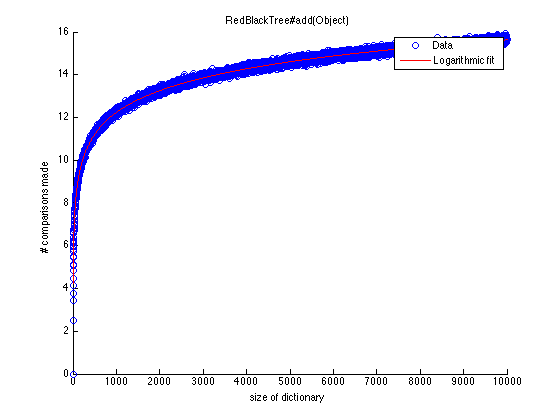
\includegraphics[width=0.49\textwidth]{resources/add}
    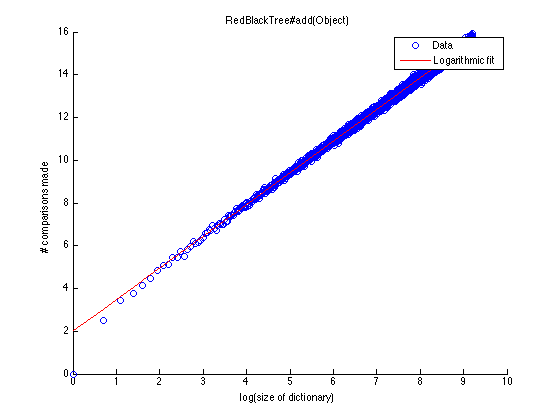
\includegraphics[width=0.49\textwidth]{resources/add_log}
    \caption{The number of comparisons made when adding a random distinct element to a dictionary of size \textit{n} (linear and log-linear scale)}

\end{figure}

\begin{figure}[!htbp]
    \centering
    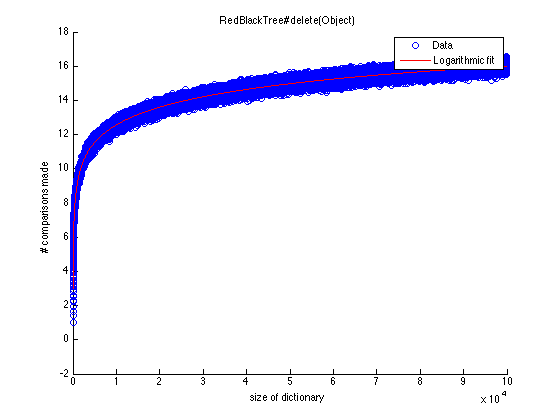
\includegraphics[width=0.49\textwidth]{resources/del}
    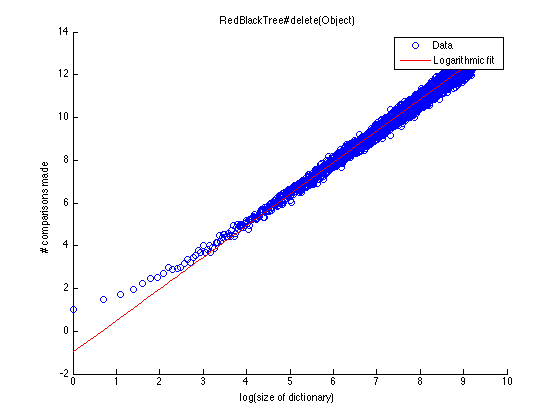
\includegraphics[width=0.49\textwidth]{resources/del_log}
    \caption{The number of comparisons made when deleting a random element from a dictionary of size \textit{n} (linear and log-linear scale)}
\end{figure}

\begin{figure}[!htbp]
    \centering
    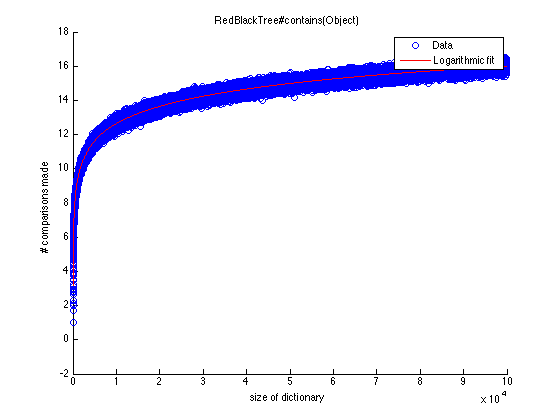
\includegraphics[width=0.49\textwidth]{resources/search}
    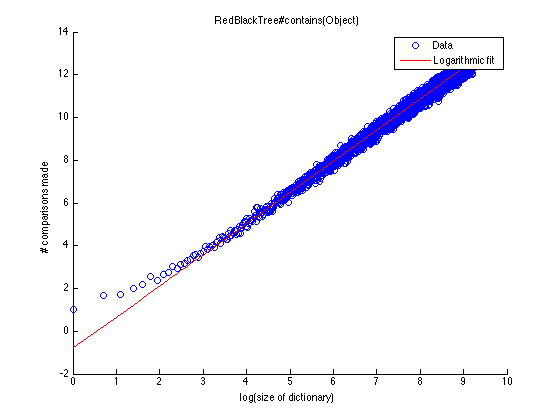
\includegraphics[width=0.49\textwidth]{resources/search_log}
    \caption{The number of comparisons made when searching for a random element in a dictionary of size \textit{n} (linear and log-linear scale)}
\end{figure}